\subsection{Model-View-Controller (MVC)} % Example for separating data and presentation

\begin{frame}
    \frametitle{\insertsubsection{} -- Targeted Problem}


\end{frame}

\begin{frame}
    \frametitle{\insertsubsection{}}
        \begin{fancycolumns}[widths={45,55}]
            \begin{definition}{Model-View-Controller}
                \begin{itemize}
                    \item Model: 
                    \item View:
                    \item Controller:
                \end{itemize}
            \end{definition}
            \nextcolumn
                \begin{figure}
                    \centering
                    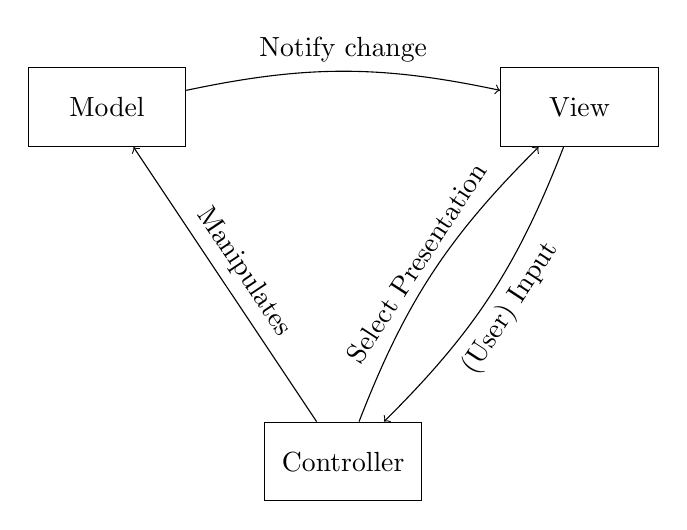
\begin{tikzpicture}
                        \node (model) at (0,0) [draw, minimum width=2cm, minimum height=1cm] {Model};
                        \node (view) at (6,0) [draw, minimum width=2cm, minimum height=1cm] {View};
                        \node (controller) at (3,-4.5) [draw, minimum width=2cm, minimum height=1cm] {Controller};
                        
                        \draw[->] (controller) to node[above, midway, sloped] {Manipulates} (model);

                        \draw[->, bend left=12] (controller) to node[ above, midway, sloped] {Select Presentation} (view);
                        \draw[->, bend left=12] (view) to node[below, midway, sloped] {(User) Input} (controller);

                        \draw[->, bend left=12] (model) to node[above, midway, sloped] {Notify change} (view);
                    \end{tikzpicture}
                \end{figure}
        \end{fancycolumns}
\end{frame}

\begin{frame}
    \frametitle{\insertsubsection{} -- Example}

\end{frame}

\subsection{Repository Architecture} % Example for organizing data storage and access

\subsection{Pipes and Filters} % Example for organizing data processing

\subsection{Microservices} % Example for organizing distributed systems

\subsection{Service-Oriented Architecture (SOA)} % Example for separating concerns in distributed systems


% Possible further architectures (obviously not exhaustive): Event-Driven Architecture (EDA), Space-Based Architecture, Client-Server, Peer-to-Peer, Publish-Subscribe, Blackboard Architecture